\section{Example}
To show how efficient code using the flyweight pattern can be compared to code not doing so, we have made a simple application, which creates rectangles containing a bitmap image in a color (red, green, or blue) and different positions (on a canvas or similar).
The bitmaps we have used is about 3 mb in size each, and it is clear that we can benefit a lot regarding memory usage if the bitmaps are shared compared to having each rectangles hold its own bitmap.
To see how much we benefit from the flyweight pattern lets take a look at the memory consumption of 250 rectangles. One using flyweight objects which contains X and Y coordinates and a reference to the bitmap (created by a factory class).
\begin{figure}[h]
\centering
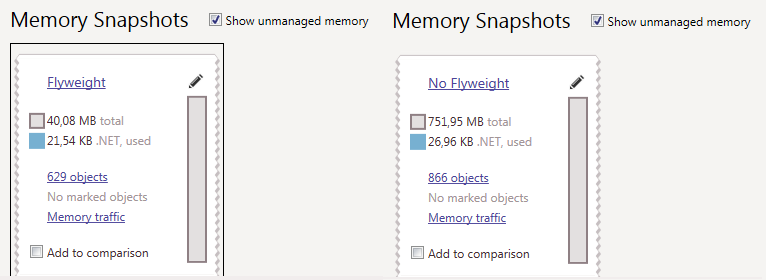
\includegraphics[width=0.7\linewidth]{Content/Flyweight_Stats}
\caption{Comparison of a normal application and one using flyweight}
\label{fig:Flyweight_Stats}
\end{figure}
It is clear to see that this application benefits a lot from the flyweight objects regarding memory consumption, but it is not only memory consumption that flyweight objects reduce, the object creation time is reduced as well. Below is shown some execution times from the application (creating 250 rectangles).
\begin{figure}[h]
\centering
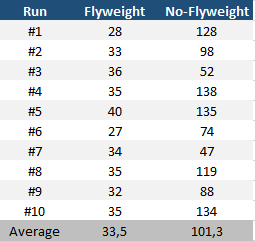
\includegraphics{Content/TimeTable}
\caption{Times it took to run the applications (in milliseconds)}
\label{fig:TimeTable}
\end{figure}
